\documentclass{standalone}
\usepackage[centertags]{amsmath}
\usepackage{latexsym}
\usepackage{amsfonts}
\usepackage{amssymb}
\usepackage{amsthm}
\usepackage{newlfont}
\usepackage{enumerate}
\usepackage{makeidx}
\usepackage{tikz}
\usetikzlibrary{backgrounds,intersections}
\begin{document}
        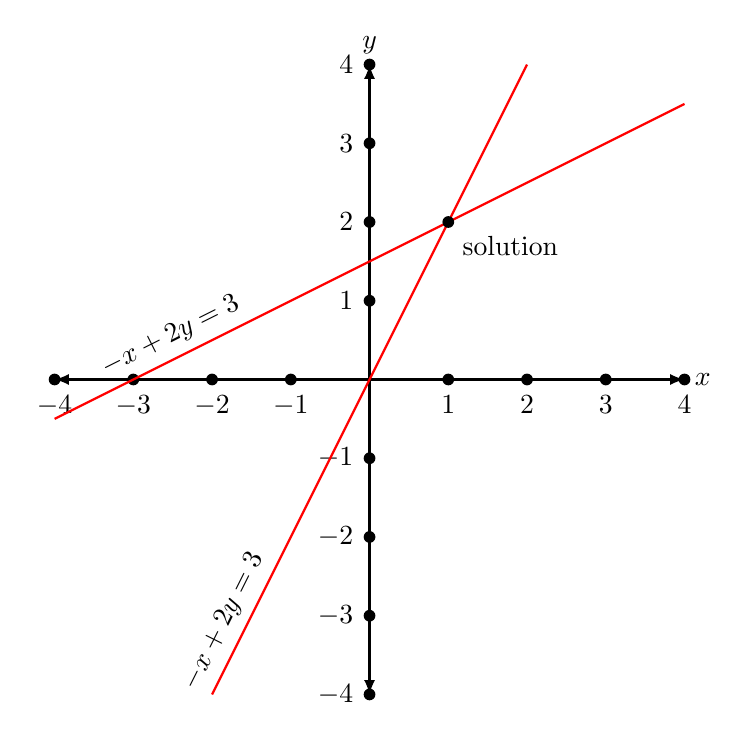
\begin{tikzpicture}
        \draw[thick,latex-latex] (-4,0) -- (4,0)node[right]{$x$};
        \draw[thick,latex-latex] (0,-4) -- (0,4)node[above]{$y$};
        \foreach \x in {-4,-3,-2,-1,1,2,3,4}{
            \node[fill,circle,inner sep=1.5pt,label=below:$\x$] at (\x,0) {};
            \node[fill,circle,inner sep=1.5pt,label=left:$\x$] at (0,\x) {};
        }
        \draw[red,thick] (-4,-0.5) -- (4,3.5)
        node[pos=0.2,black,above,sloped] {$-x+2y=3$};
        \draw[red,thick] (-2,-4) -- (2,4)
        node[pos=0.1,black,above,sloped] {$-x+2y=3$};
		\node[fill,circle,inner sep=1.5pt,label=below right:solution] at (1,2) {};

        \end{tikzpicture}
\end{document}
